%! TeX program = lualatex
\documentclass[main]{subfiles}

\begin{document}

\title[AutoML: BO]{Acquisition Function Optimization}
\subtitle{Finding the Next Candidate Point}
\author[Bernd Bischl]{Bernd Bischl}
\date{}

\titlebackground*{images/AutoML_HPO_2_2}

    \maketitle


\begin{frame}[t]{Why Optimize the Acquisition Function?}
  \begin{itemize}
    \item BO's inner loop has \emph{two} optimization problems:
        \begin{itemize}
            \item \textbf{Outer:} (expensive) evaluations of $\cost$ -- driven by the acquisition function
            \item \textbf{Inner:} find $\confI{t+1} = \argmax_{\conf \in \pcs} \acq(\conf)$ -- only uses the surrogate and costs CPU time
        \end{itemize}
    \item Acquisition function evaluations are \textbf{cheap} (forward pass through surrogate) -- but the inner problem is still non-trivial
    \item A poor inner optimizer gives BO a bad candidate, wastes an expensive $\cost$ evaluation
  \end{itemize}
  \vspace{0.2cm}
  \begin{center}
  \textbf{Good inner optimization is crucial for BO performance.}
  \end{center}
\end{frame}


\begin{frame}[t]{The Acquisition Function Landscape}
  \begin{itemize}
    \item $\acq$ is typically \textbf{non-convex} and \textbf{multi-modal}
    \item For EI / PI: $\acq(\conf) = 0$ at training points; peaks sit between them
    \item Landscape gets more rugged as the surrogate is fit to more data
    \item In high dimensions: flat plateaus with narrow peaks -- hard to find
  \end{itemize}
  \vspace{0.2cm}
  \begin{center}
    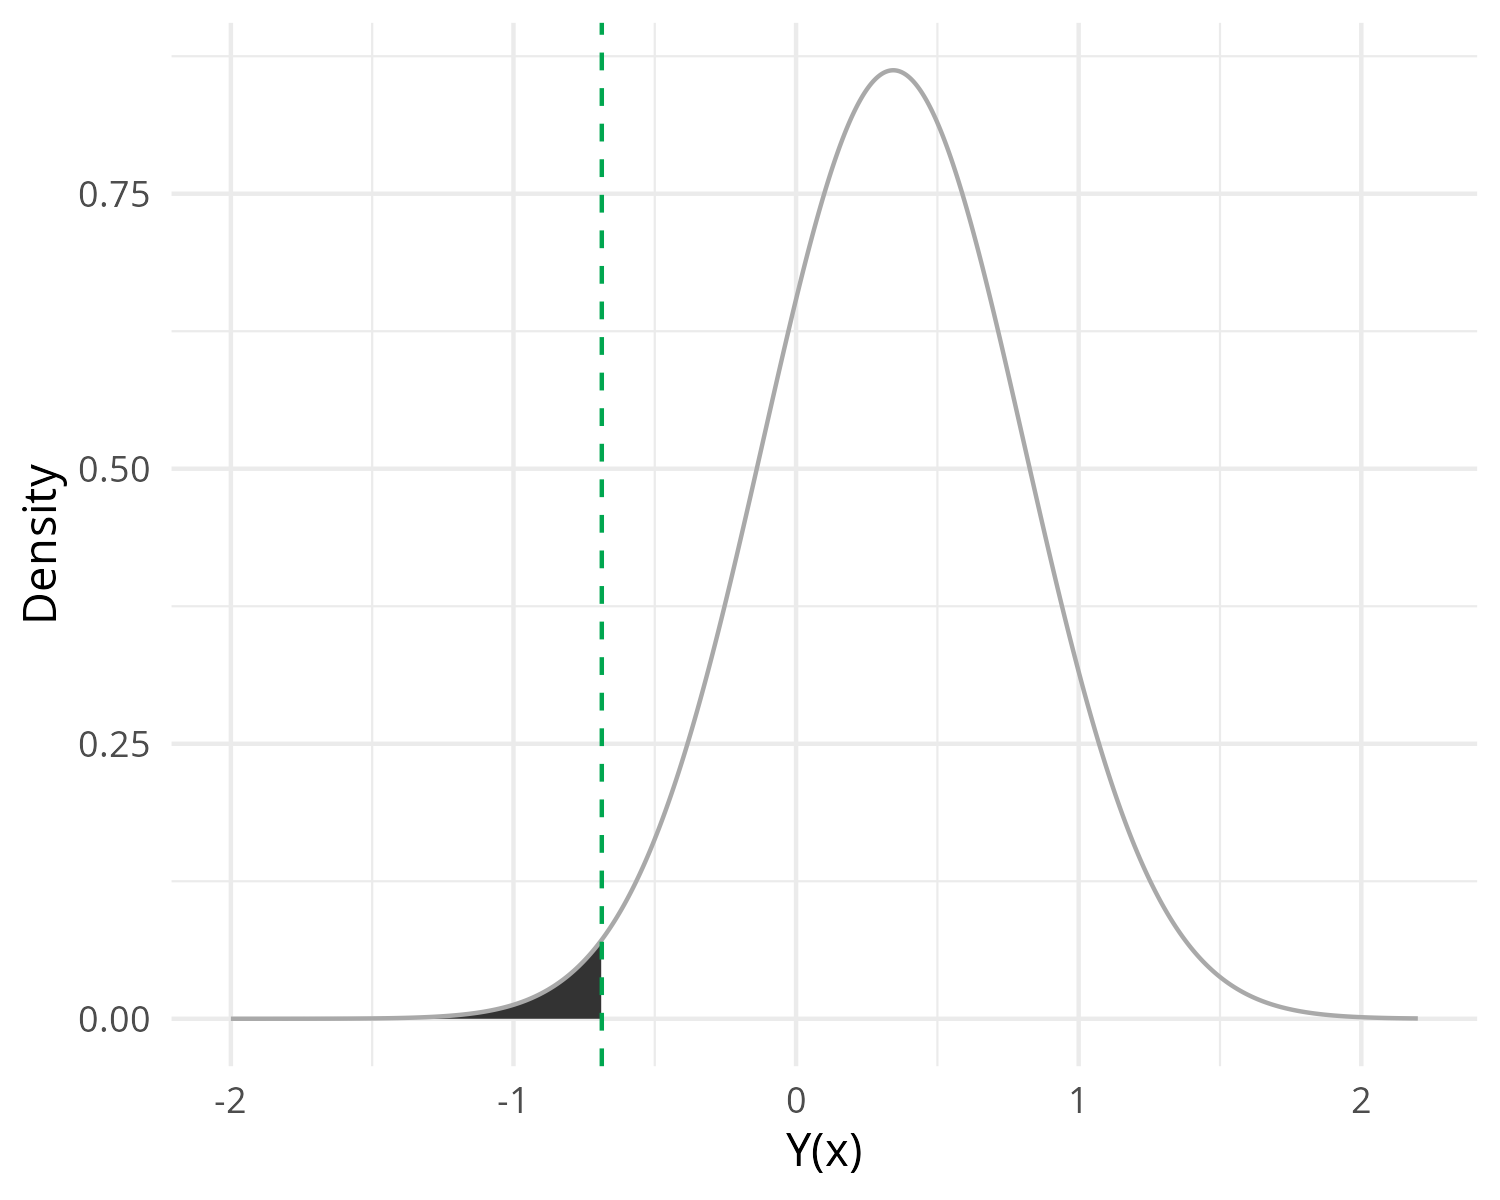
\includegraphics[width=.65\textwidth]{images/bayesian_loop_pi_0.png}\\
    \footnotesize Example: a PI landscape in 1D -- several peaks, zeros at observed points.
  \end{center}
\end{frame}


\begin{frame}[t]{Numeric Search Spaces}
  \begin{itemize}
    \item \textbf{Multi-start local search:}
        \begin{itemize}
            \item Sample many start points (uniform / LHS / Sobol)
            \item Run gradient-based local optimizer from each (L-BFGS-B if $\pcs$ is box-constrained)
            \item Return the best local optimum
        \end{itemize}
    \item Gradients through the acquisition function:
        \begin{itemize}
            \item GP surrogate: $\surro(\conf)$ and $\sh(\conf)$ are differentiable $\leadsto$ closed-form $\nabla \acq$
            \item Random forest surrogate: piecewise constant $\leadsto$ no gradients, use gradient-free methods
        \end{itemize}
    \item \textbf{DIRECT} (DIviding RECTangles): deterministic, no gradients; covers the box systematically -- nice for low-$d$
  \end{itemize}
\end{frame}


\begin{frame}[t]{Mixed / Hierarchical Search Spaces}
  \begin{itemize}
    \item Many AutoML spaces mix continuous, integer, categorical, and \emph{conditional} HPs
    \item Gradients no longer meaningful $\leadsto$ gradient-based methods fail
    \item Common choices:
        \begin{itemize}
            \item \textbf{Random search} with large sample -- cheap, trivially parallel, easy baseline
            \item \textbf{Evolutionary / local search} (e.g.\ focused search in SMAC): mutate current best along one HP at a time
            \item \textbf{Interleaved}: random sampling + local refinement on the best candidates
        \end{itemize}
    \item Respect conditional structure: only mutate an HP if its parent choice activates it
  \end{itemize}
\end{frame}


\begin{frame}[t]{Budget and Restarts}
  \begin{itemize}
    \item Acquisition optimization has its own \textbf{budget}: \# starts $\times$ iterations per start
    \item Trade-off:
        \begin{itemize}
            \item Too few restarts $\leadsto$ miss the global peak, propose suboptimal points
            \item Too many restarts $\leadsto$ overhead per BO iteration grows (problematic when $\cost$ is cheap-ish, e.g.\ small HPO benchmarks)
        \end{itemize}
    \item Typical defaults: $10$--$50$ restarts for GP + L-BFGS-B in $\le 20$ dimensions
    \item Scale budget with $d$: higher-dimensional landscapes need more starts
  \end{itemize}
\end{frame}


\begin{frame}[t]{Parallel / Batch Proposals}
  \begin{itemize}
    \item Often we can evaluate $\cost$ on several points in parallel (HPC, multi-GPU, lab experiments)
    \item Need to propose $q > 1$ candidates at once, not just $\confI{t+1}$
    \item Approaches:
        \begin{itemize}
            \item \textbf{$q$-acquisition functions} ($q$EI, $q$UCB): joint expectation over a batch of $q$ points -- estimated via Monte Carlo
            \item \textbf{Sequential fantasizing}: propose one point, ``pretend'' its outcome ($\sim$ surrogate posterior), refit, propose next
            \item \textbf{Penalization / local penalization}: after picking a point, down-weight the AF in its neighborhood to force diversity
        \end{itemize}
    \item Batch optimization is now a much higher-dimensional inner problem ($q \cdot d$)
  \end{itemize}
\end{frame}


\begin{frame}[t]{When Inner Optimization Matters Most}
  \begin{itemize}
    \item \textbf{Expensive $\cost$:} each evaluation is minutes-to-hours -- worth spending CPU on careful inner optimization
    \item \textbf{Late in the BO run:} surrogate is well-trained, AF peaks are narrow -- easy to miss
    \item \textbf{Noisy / multi-objective:} AF is stochastic / vector-valued -- needs specialized inner optimizers
  \end{itemize}
  \vspace{0.2cm}
  \begin{itemize}
    \item When \emph{not} to over-engineer:
        \begin{itemize}
            \item $\cost$ is cheap and many BO iterations are planned $\leadsto$ save overhead with simpler inner search
            \item Low-dim, smooth surrogate $\leadsto$ a short L-BFGS-B with $\sim\!5$ restarts is enough
        \end{itemize}
  \end{itemize}
\end{frame}


\begin{frame}[t]{Summary}
  \begin{enumerate}
    \item BO's inner loop is itself an optimization problem -- but over the \emph{cheap} surrogate
    \item The AF landscape is non-convex, multi-modal, and gets rugged with more data
    \item Numeric spaces: multi-start L-BFGS-B (w/ GP gradients) or DIRECT
    \item Mixed / hierarchical spaces: random search, evolutionary search, or hybrids
    \item Batch / parallel BO needs $q$-acquisition functions or fantasizing / penalization
    \item Budget and restarts scale with problem dimensionality
  \end{enumerate}
\end{frame}


\end{document}
